\section{Introduction}
\label{sec:intro}
% intro to the use of discussion models
Text-to-image models have enabled the possibility of generating personalized images with the content described by words, transforming industries, and even, our thoughts. Given these models’ impact on our lives, it is key to guarantee they are developed responsibly, battling stereotypes \cite{bloomberg, SolbesCanales2020SocializationOG}, lack of diversity, and inherited biases, but remaining truthful \cite{verge2024gemini}. Moreover, if this biased generated data is used for training future models, these biases will persist or be amplified in the new models themselves. 

 %On top of all, we still fail to completely understand the results of our generations, which in many cases tend to be disappointing, diverging from expectations, and requiring highly detailed prompts for successful outputs. Moreover, a gap exists in Explainable Generative AI to facilitate the understanding of concept relationships. Identifying these biases and relationships represents an initial phase in determining which ones require mitigation and will be addressed. 

%This work aims to address a specific area for improvement in the field, amidst a wide range of ongoing research efforts: understanding concept relationships in text-to-image generations and combating bias.

%In this work, we treat relationships as simply neutral associations between concepts, while biases deviate from objectivity, leading to skewed perceptions with unfair inclinations or prejudices. 

%It is key to understand the difference between relationships and biases. The former are associations between two or more concepts, that can be neutral such as the concept of \textit{CEO} being associated to the attribute \textit{suit}, or \textit{water} being connected to the concept of \textit{waterbird}. On the other hand, biases will be treated as a deviation from an objective representation. It can refer to any inclination or prejudice for or against an individual, group, or idea, often in a way considered to be unfair. Biases can skew perceptions and prevent a fair or accurate understanding of a concept, leading to a distorted perception, and unfair treatment.



%As a result of the above, the main research objective is addressing the need for global data representation,
%by concepts’ relationship understanding and bias mitigation in diffusion models.

%Through this empirical analysis, we address these
%research questions and contribute the following:
%-----------------------------------------------------------

\begin{figure}[t]
  \centering
   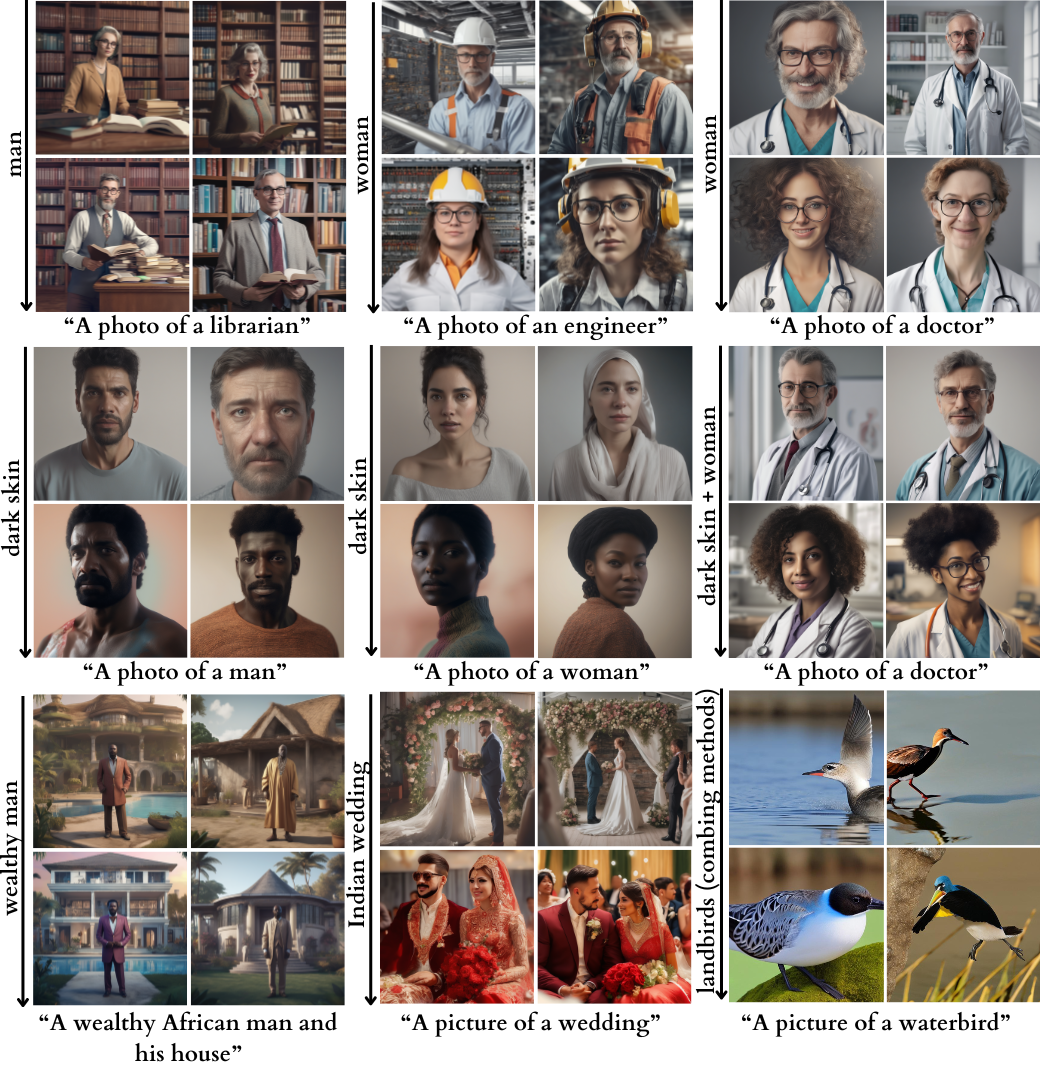
\includegraphics[width=1\linewidth]{images/original_2.png}
   \caption{\textbf{Debiasing diverse concepts.} Generations observed upon the application of our approach in several scenarios.  }
   \label{fig:debiasing_results}
\end{figure}

%The analysis of biases within generative models reveals pervasive biases ranging from gender and race to geographic representation. Notably, Leonardo N. and Dina B. identified concerning patterns in Stable Diffusion v1.5 where low-paying jobs are disproportionately represented by women and darker-skinned individuals. While much research focuses on social and racial biases, Basu et al. conducted a user study validating geographical biases in models like DALLE 2 and Stable Diffusion. Cultural biases were also found, such as in homoglyphs in text-to-image synthesis, where specific characters lead to cultural biases in generated images. Efforts to understand and mitigate biases in vision-language models involve automated gender estimation, face and skin tone detection, and evaluation of geographical representativeness using CLIP-based similarity and k-nearest neighbor models. Debiasing efforts include interventions in prompts, altering prompt embeddings, and leveraging external attribute datasets. Chuang et al.'s method shows promise in improving diversity but operates under assumptions that may not universally hold, while Zhang et al.'s ITI-Gen requires specific attribute datasets and struggles with certain debiasing tasks.

From gender to race, to poor geographic representation, biases can be found everywhere in generative models. Leonardo N. and Dina B. \cite{bloomberg} have found a concerning pattern in Stable Diffusion v1.5 where low-paying jobs are dominated by women and darker-skinned individuals. While most of the work focuses on social and racial biases \cite{bolukbasi2016man, xu2018fairgan}, Basu \textit{et al.} \cite{basu2023inspecting} conduct a user study validating geographical biases in models like DALLE \cite{ramesh2021zeroshot} and Stable Diffusion \cite{rombach2022highresolution}, finding underrepresented 25 out of 27 countries. Cultural biases are also found when using homoglyphs in text-to-image synthesis \cite{mikolov2013exploiting}. Efforts to understand biases in vision-language models lead to the development of automated tools \cite{cho2023dalleval, luccioni2023stable}, the use of gender estimation \cite{li2023blip2}, face and skin tone detection \cite{Bulat_2017, feng2022racially}, and the evaluation of geographical representativeness using CLIP-based similarity and k-nearest neighbor models \cite{basu2023inspecting}. Mitigation efforts include prompt interventions \cite{bansal2022texttoimage}, the development of more inclusive datasets featuring images reflecting diverse geographic and socioeconomic contexts \cite{NEURIPS2022_5474d9d4, ramaswamy2023geode}, and alterations in prompt embedding strategies \cite{chuang2023debiasing, zhang2023itigen}. Chuang \textit{et al.} \cite{chuang2023debiasing} propose a method to mitigate bias by maximizing the similarity between biased and non-biased prompts. They construct a projection matrix to eliminate biased directions from text embeddings before inputting them into the model. Using a similar approach, but employing tokens of available image datasets, ITI-Gen \cite{zhang2023itigen} learns a set of prompt embeddings to append to the initial prompt.

%However, it operates under the assumption the closer the similarity between two text prompts and their embeddings, the more equally represented they should appear on the generated images, which is not a universal truth, being considered a limitation. 


%\textbf{Understanding Vision Language Models.} In an attempt to understand biases in an automated way, Cho \textit{et al.} \cite{cho2023dalleval} use BLIP-2 \cite{li2023blip2} for gender estimation, and FAN \cite{Bulat_2017} and TRUST \cite{feng2022racially} for face and skin tone detection. For automatic evaluation of geographical representativeness, Basu \textit{et al.} \cite{basu2023inspecting} propose CLIP-based similarity between the country specific prompt and the generated image, and k-nearest neighbor model assessing the similarity between a test image and previously annotated images. Luccioni, A. S. \textit{et al.} \cite{luccioni2023stable} introduce three tools to guide in-depth model analysis across biases in professions, a Diffusion Bias Explorer, an Average Face Comparison Tool and two nearest-neighbor lookup tools.

%\textbf{Debiasing Vision Language Models}.  Certain efforts have been directed towards creating more inclusive datasets where images representing geographic and socioeconomic diversity are gathered \cite{NEURIPS2022_5474d9d4, ramaswamy2023geode}. Bansal \textit{et al.} \cite{bansal2022texttoimage} inject ethical interventions into the prompt, such as ”if all individuals can be a [profession] irrespective of their gender”, as a method for combating bias. The state-of-the-art advancements in bias mitigation without requiring additional training or hard prompting, focus on the alteration of prompt embeddings to condition the generations. In these lines, Chuang \textit{et al.} \cite{chuang2023debiasing} maximize the similarity between biased and nonbiased prompts to construct a projection matrix that projects out those biased directions, applied to the text embeddings before feeding them into the model. Their method improves diversity both in their experiments with gender and race, but also generating waterbirds in nonwater backgrounds. However, it operates under the assumption the closer the similarity between two text prompts and their embeddings, the more equally represented they should appear on the generated images, which is not a universal truth, being considered a limitation. In addition to novel work, Zhang \textit{et al.} present ITI-Gen \cite{zhang2023itigen}, leveraging external attribute datasets to learn inclusive tokens that can be combined with the prompt’s embeddings. While the method showcases promising results, it requires a solid dataset of the specific debiasing attribute, failing to handle our experiments debiasing skin tone for the prompt ”A wealthy African man and his house”, proposed by \cite{sunandopaper}, or the Waterbirds benchmark. 

We first present a tool to enhance developers’ visibility, given that we believe understanding the relationship between concepts, and the reason for certain attributes appearing in generations, is key to mitigating them. Secondly, we propose a straightforward novel approach for bias mitigation, linearly separating the latents, noisy information tensors of two different prompts, learning the transformation for debiasing in the latent space of the diffusion model. 

We apply this transformation, named \textit{latent direction}, at a specific weight, linearly combining it with the initial Gaussian noise. The results in a series of diverse experiments prove it successfully works to debias, without the need for prompt alteration. Our approach remains simple, while effective and adaptable to varied scenarios. It allows the synergy of different latent directions, and it is flexible to be used in combination with an approach modifying the prompt embeddings if desired. Through our experiments, we focus on demonstrating the impact of our method for the maximum debiasing transition. However, fair distributions\footnote{Distribution of the generations selected by the user with ethical, truthful, and responsible considerations in mind.} can be obtained when applying the learned latent direction to only a determined percentage of the generations.
 
